\clearpage
\subsection{premi/client/trailMap}
\begin{figure}[H]
\begin{center}
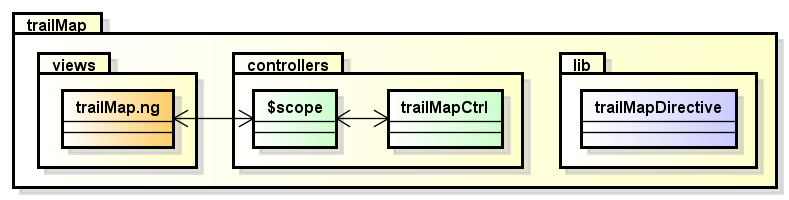
\includegraphics[scale=0.70]{img/diapkg/trailMap.png}
\caption{Diagramma della classe premi/client/trailMap}
\end{center}
\end{figure}

%-------  diagramma di un template %
\subsubsection{premi/client/trailMap/views/trailMap.ng}

\begin{description}
%-------  descrizione del template%
\item[Descrizione] \hfill
	Template della vista associata allo \textit{\$scope} di \textit{trailMapCtrl} che visualizza una mappa per un determinato trail. Nella sezione Frames Out sono presenti i frame che non sono presenti nel trail e che possono essere aggiunti. Nella sezione Trail è presente un menù che permette di aggiungere un checkpoint e di aggiungere i frame nel trail. 
\end{description}

%-------  diagramma della classe%
\subsubsection{premi/client/trailMap/controllers/trailMapCtrl}
\begin{figure}[H]
\begin{center}
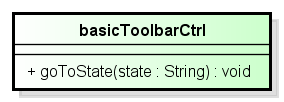
\includegraphics[scale=0.85]{img/diacla/basicToolbarCtrl.png}
\caption{Diagramma della classe premi/editor/controllers/basicToolbarCtrl}
\end{center}
\end{figure}


\begin{description}
%-------  descrizione della classe%
\item[Descrizione] \hfill
	Controller della view \textit{basicToolbar.ng}. Fornisce, tramite lo \textit{\$scope} un metodo per passaggio da un editor all'altro
	\\ La dicitura \{\$scope\} nel diagramma UML$_G$ indica che:
\begin{itemize}
\item tutti gli attributi e i metodi pubblici del controller vanno inseriti nello \$scope;
\item tutti gli attributi e i metodi privati del controller appartengono al controller.
\end{itemize}
Vedere la sezione \ref{servizi} per approfondimenti sull'oggetto \$scope.
	
%-------  lista dei metodi%	
\item[Metodi] \hfill

	% -- inizio metodo -- %
	\begin{description}
		\item[\textbf{\color{blue}+ goToState(state : String) : void			}] \hfill
			Tramite il metodo \textit{\$state.go} cambia "stato" dell'editor, passando da una fase di creazione della presentazione all'altra.
			
		\begin{description}
			% -- lista argomenti del metodo -- %
			\item[Argomenti] \hfill
				\begin{itemize}
				
					\item \textbf{state : String			} \hfill
					Il nuovo stato dell'editor. Gli stati dell'editor al momento sono:
					\begin{itemize}
						\item "premi.editor.frame"
						\item "premi.editor.infographic"
						\item "premi.editor.trails"
					\end{itemize}
					
				\end{itemize}
		\end{description}
	\end{description}
	% -- fine metodo -- %
	
	% -- inizio metodo -- %
	\begin{description}
		\item[\textbf{\color{blue}+ activeStateClass(state : String) : String			}] \hfill
			Verifica se un determinato stato è attivo. Restituisce "active" nel caso lo stato sia attivo altrimenti restituisce una stringa vuota.
			
		\begin{description}
			% -- lista argomenti del metodo -- %
			\item[Argomenti] \hfill
				\begin{itemize}
				
					\item \textbf{state : String			} \hfill
					identifica il nome dello stato da controllare.
					
				\end{itemize}
		\end{description}
	\end{description}
	% -- fine metodo -- %	
		
\end{description}
